\section{Blending and the infinite}
\label{sec:infinity}

\note{Marco, Ewen, Alan, Felix}


In this paper we want to follow Goguen's proposal \cite{Go99c} for
implementing blending, but slightly simplified (like in
\cite{KuMoHoBhBa12}): we will only deal with
the well-known notion of colimit in a category \cite{Gog91}, instead of
using $\frac{3}{2}$-colimits.

In the examples here considered we will be using colimits of V-shaped
diagrams (cf.~Figure??). Thus, in each of the cases we have to specify
two morphisms between a source conceptual space and a target conceptual
space, with the restriction that both morphisms share the same source
conceptual space.

Additionally we will assume that the involved conceptual spaces are
always given using a
CASL specification \cite{MoHaSaTa08} and that the morphisms are theorem
preserving (but perhaps not axiom preserving). The reason to these
assumptions
is that in these cases it is well-known how to compute colimits
\cite{Mo98a}; the colimit specification essentially corresponds to the
disjoint union of the two target conceptual spaces except for not
repeating the symbols given in the common source conceptual space.
Moreover, we will be using 
the HETS system \parencite{MossakowskiEA06} to compute such colimits.



\subsection{Naturals and Integers}

\subsection{Example Revisited -- the Integers}

As a first demonstration of the machinery involved in blending
mathematical theories, we consider combining a theory of natural
numbers with the concept of the inverse of a function to obtain the
integers. Let us assume an simple axiomatisation of the natural
numbers (without order axioms) as shown in Figure \ref{fig:nats}, and
call this theory $\SIdIndex{Nat}$. Now let us also define a simple theory
which introduces the concept of a function with an inverse as shown in
Figure \ref{fig:inv}, and call this theory $\mathbb{F}$. 
\begin{figure}[!ht]
\begin{hetcasl}
\SPEC \=\SIdIndex{Nat} \Ax{=}\\
\> \SORT \Id{Nat}\\
\> \OPS \=\Id{zero} \Ax{:} \Id{Nat};\\
\>\> \Id{s} \Ax{:} \=\Id{Nat} \Ax{\rightarrow} \Id{Nat};\\
\>\> \Ax{\_\_}\Ax{+}\Ax{\_\_} \Ax{:} \=\Id{Nat} \Ax{\times} \Id{Nat} \Ax{\rightarrow} \Id{Nat}\\
\> \Ax{\forall} \=\Id{x}, \Id{y}, \Id{z} \Ax{:} \Id{Nat} \\
\> \Ax{\bullet} \=\Id{s}(\Id{x}) \Ax{=} \Id{y} \Ax{\wedge} \=\Id{s}(\Id{x}) \Ax{=} \Id{z} \Ax{\Rightarrow} \=\Id{y} \Ax{=} \Id{z}\\
\> \Ax{\bullet} \=\Id{s}(\Id{x}) \Ax{=} \Id{s}(\Id{y}) \Ax{\Rightarrow} \=\Id{x} \Ax{=} \Id{y}\\
\> \Ax{\bullet} \=\Ax{\exists} \Id{a} \Ax{:} \Id{Nat} \Ax{\bullet} \=\Id{s}(\Id{x}) \Ax{=} \Id{a}\\
\> \Ax{\bullet} \Ax{\neg} \=\Id{s}(\Id{x}) \Ax{=} \Id{zero}\\
\> \Ax{\bullet} \=\Id{s}(\Id{x}) \Ax{+} \Id{y} \Ax{=} \Id{s}(\=\Id{x} \Ax{+} \Id{y})\\
\> \Ax{\bullet} \=\Id{zero} \Ax{+} \Id{y} \Ax{=} \Id{y}\\
\KW{end}
\end{hetcasl}
\caption{A theory of the natural numbers without order}
\label{fig:nats}
\end{figure}

\begin{figure}[!ht]
\begin{hetcasl}
\SPEC \=\SIdIndex{Func} \Ax{=}\\
\> \SORT \Id{X}\\
\> \OP \=\Id{f} \Ax{:} \=\Id{X} \Ax{\rightarrow} \Id{X}\\
\> \OP \=\Id{finv} \Ax{:} \=\Id{X} \Ax{\rightarrow} \Id{X}\\
\> \Ax{\forall} \=\Id{x} \Ax{:} \Id{X} \\
\> \Ax{\bullet} \=\Id{f}(\Id{finv}(\Id{x})) \Ax{=} \Id{x}\\
\> \Ax{\bullet} \=\Id{finv}(\Id{f}(\Id{x})) \Ax{=} \Id{x}\\
\KW{end}
\end{hetcasl}
\caption{A theory with a function and its inverse defined}
\label{fig:inv}
\end{figure}



\subsubsection{Identifying a Generic Space}
In order to incorporate the notion of blending here we want to be able
to identify a ``generic'' component of each theory and compute the
colimit (also known as pushout) as discusses in \S\ref{sec:background}. We can use the
HDTP system \parencite{GustKS2006,Schmidt2010} to discover a common theory
and signature morphism between symbols in the
two theories $\SIdIndex{Nat}$ and $\SIdIndex{Fun}$. The Generic theory
contains a sort $N$ and a function $func$, and the morphisms from the
Generic theory to $\SIdIndex{N}$ and $\SIdIndex{Fun}$ are:
\begin{align}
s&&\leftarrow_{g_\SIdIndex{Nat}}&&func&&\rightarrow_{g_\SIdIndex{Fun}}&&f\\
Nat&&\leftarrow_{g_\SIdIndex{Nat}}&&N&&\rightarrow_{g_\SIdIndex{Fun}}&&X
\end{align}
Here the successor function is identified in the mapping with the
function in the theory $\SIdIndex{Fun}$, and $g_K$ is the label for
the set of symbol mappings determined by the signature morphism from
the Generic space the theory $K$.

\subsubsection{Computing the Colimit}
The HETS system \parencite{MossakowskiEA06} can then be exploited to
find a new theory by computing the colimit:
\begin{center}
  \begin{diagram}[size=7mm]
    &       &   $Gen$   &       & \\
    & \ldTo^{\rotatebox{-45}{$g_\SIdIndex{Nat}$}} &       &
    \rdTo^{\rotatebox{45}{$g_\SIdIndex{Fun}$}} &          \\
    \SIdIndex{Nat} &       &   &       & \SIdIndex{Fun} \\
    & \rdTo_{\rotatebox{45}{$b_\SIdIndex{Nat}$}} &       &
    \ldTo_{\rotatebox{-45}{$b_\SIdIndex{Fun}$}} &  \\
    & & $Blend$ & &
  \end{diagram}
\end{center}
This generates the theory shown in \ref{fig:inconsistentintegers}.

\begin{figure}[!ht]
\begin{hetcasl}
\SPEC \=\SIdIndex{Spec} \Ax{=}\\
\> \SORT \Id{N}\\
\> \OP \=\Ax{\_\_}\Ax{+}\Ax{\_\_} \Ax{:} \=\Id{N} \Ax{\times} \Id{N} \Ax{\rightarrow} \Id{N}\\
\> \OP \=\Id{p} \Ax{:} \=\Id{N} \Ax{\rightarrow} \Id{N}\\
\> \OP \=\Id{s} \Ax{:} \=\Id{N} \Ax{\rightarrow} \Id{N}\\
\> \OP \=\Id{zero} \Ax{:} \Id{N}\\
\> \Ax{\forall} \=\Id{x}, \Id{y}, \Id{z} \Ax{:} \Id{N} \=\Ax{\bullet} \=\Id{s}(\Id{x}) \Ax{=} \Id{y} \Ax{\wedge} \=\Id{s}(\Id{x}) \Ax{=} \Id{z} \Ax{\Rightarrow} \=\Id{y} \Ax{=} \Id{z} \`{\small{}\KW{\%}(Ax1)\KW{\%}}\\
\> \Ax{\forall} \=\Id{x}, \Id{y} \Ax{:} \Id{N} \=\Ax{\bullet} \=\Id{s}(\Id{x}) \Ax{=} \Id{s}(\Id{y}) \Ax{\Rightarrow} \=\Id{x} \Ax{=} \Id{y} \`{\small{}\KW{\%}(Ax2)\KW{\%}}\\
\> \Ax{\forall} \=\Id{x} \Ax{:} \Id{N} \=\Ax{\bullet} \=\Ax{\exists} \Id{a} \Ax{:} \Id{N} \Ax{\bullet} \=\Id{s}(\Id{x}) \Ax{=} \Id{a} \`{\small{}\KW{\%}(Ax3)\KW{\%}}\\
\> \Ax{\forall} \=\Id{x} \Ax{:} \Id{N} \=\Ax{\bullet} \Ax{\neg} \=\Id{s}(\Id{x}) \Ax{=} \Id{zero} \`{\small{}\KW{\%}(Ax4)\KW{\%}}\\
\> \Ax{\forall} \=\Id{x}, \Id{y} \Ax{:} \Id{N} \=\Ax{\bullet} \=\Id{s}(\Id{x}) \Ax{+} \Id{y} \Ax{=} \Id{s}(\=\Id{x} \Ax{+} \Id{y}) \`{\small{}\KW{\%}(Ax5)\KW{\%}}\\
\> \Ax{\forall} \=\Id{y} \Ax{:} \Id{N} \=\Ax{\bullet} \=\Id{zero} \Ax{+} \Id{y} \Ax{=} \Id{y} \`{\small{}\KW{\%}(Ax6)\KW{\%}}\\
\> \Ax{\forall} \=\Id{x} \Ax{:} \Id{N} \=\Ax{\bullet} \=\Id{s}(\Id{p}(\Id{x})) \Ax{=} \Id{x} \`{\small{}\KW{\%}(Ax1\Ax{\_}7)\KW{\%}}\\
\> \Ax{\forall} \=\Id{x} \Ax{:} \Id{N} \=\Ax{\bullet}
\=\Id{p}(\Id{s}(\Id{x})) \Ax{=} \Id{x}
\`{\small{}\KW{\%}(Ax2\Ax{\_}8)\KW{\%}}
\end{hetcasl}
\caption{An inconsistent version of the integers (without order)}
\label{fig:inconsistentintegers}
\end{figure}


\subsubsection{Removal of Inconsistencies}
This theory is automatically determined to be inconsistent due to the axioms
\begin{eqnarray}
\forall x : \mathbb{Z} . not s(x) &=& 0 \label{eq:limnat1}\\
s(p(x)) &=& x \label{eq:sucpre}
\end{eqnarray}
Removal of the limiting axiom (\ref{eq:limnat1}) results in a theory which is very
similar to what we understand to be the integers as shown in Figure~\ref{fig:integers}.
\begin{figure}[!ht]
\begin{hetcasl}
\SPEC \=\SIdIndex{Spec} \Ax{=}\\
\> \SORT \Id{N}\\
\> \OP \=\Ax{\_\_}\Ax{+}\Ax{\_\_} \Ax{:} \=\Id{N} \Ax{\times} \Id{N} \Ax{\rightarrow} \Id{N}\\
\> \OP \=\Id{p} \Ax{:} \=\Id{N} \Ax{\rightarrow} \Id{N}\\
\> \OP \=\Id{s} \Ax{:} \=\Id{N} \Ax{\rightarrow} \Id{N}\\
\> \OP \=\Id{zero} \Ax{:} \Id{N}\\
\> \Ax{\forall} \=\Id{x}, \Id{y}, \Id{z} \Ax{:} \Id{N} \=\Ax{\bullet} \=\Id{s}(\Id{x}) \Ax{=} \Id{y} \Ax{\wedge} \=\Id{s}(\Id{x}) \Ax{=} \Id{z} \Ax{\Rightarrow} \=\Id{y} \Ax{=} \Id{z} \`{\small{}\KW{\%}(Ax1)\KW{\%}}\\
\> \Ax{\forall} \=\Id{x}, \Id{y} \Ax{:} \Id{N} \=\Ax{\bullet} \=\Id{s}(\Id{x}) \Ax{=} \Id{s}(\Id{y}) \Ax{\Rightarrow} \=\Id{x} \Ax{=} \Id{y} \`{\small{}\KW{\%}(Ax2)\KW{\%}}\\
\> \Ax{\forall} \=\Id{x} \Ax{:} \Id{N} \=\Ax{\bullet} \=\Ax{\exists} \Id{a} \Ax{:} \Id{N} \Ax{\bullet} \=\Id{s}(\Id{x}) \Ax{=} \Id{a} \`{\small{}\KW{\%}(Ax3)\KW{\%}}\\
\> \Ax{\forall} \=\Id{x}, \Id{y} \Ax{:} \Id{N} \=\Ax{\bullet} \=\Id{s}(\Id{x}) \Ax{+} \Id{y} \Ax{=} \Id{s}(\=\Id{x} \Ax{+} \Id{y}) \`{\small{}\KW{\%}(Ax4)\KW{\%}}\\
\> \Ax{\forall} \=\Id{y} \Ax{:} \Id{N} \=\Ax{\bullet} \=\Id{zero} \Ax{+} \Id{y} \Ax{=} \Id{y} \`{\small{}\KW{\%}(Ax5)\KW{\%}}\\
\> \Ax{\forall} \=\Id{x} \Ax{:} \Id{N} \=\Ax{\bullet} \=\Id{s}(\Id{p}(\Id{x})) \Ax{=} \Id{x} \`{\small{}\KW{\%}(Ax1\Ax{\_}7)\KW{\%}}\\
\> \Ax{\forall} \=\Id{x} \Ax{:} \Id{N} \=\Ax{\bullet} \=\Id{p}(\Id{s}(\Id{x})) \Ax{=} \Id{x} \`{\small{}\KW{\%}(Ax2\Ax{\_}8)\KW{\%}}\\
\KW{end}
\end{hetcasl}
\caption{A consistent version of the integers (without order)}
\label{fig:integers}
\end{figure}

\subsubsection{Running the Blend}

Running the blend refers to discovering axioms or definitions which
make the blend incomplete. In the example of the version in Figure
\ref{fig:integers}, the definition of plus needs to be extended to
understand how to calculate with the predecessor function:
$$
p(x) + y = p(x+y)
$$
\noindent from which theorems such as 
$$
p(x) + s(y) = x+y
$$
\noindent can be proved.


\subsection{Potential and actual infinity}

The work of \textcite{Lak00} provides a wide range of examples of
metaphorical reasoning in mathematics, while stressing the embodied
cognition involved in basic mathematical experience.  Some of
the ideas have been reworked by the authors, increasing the emphasis on
conceptual blending as central.  In particular, the analysis of
mathematical infinity, given in metaphorical form as the ``Basic Metaphor
of Infinity'' (BMI) in \textcite{Lak00}, is represented in blend form
in \textcite{nunez05} as the ``Basic Mapping of Infinity'' (so, still ``BMI'').

We show here how this blend works out in our setting.

\begin{figure}[h]
  \centering
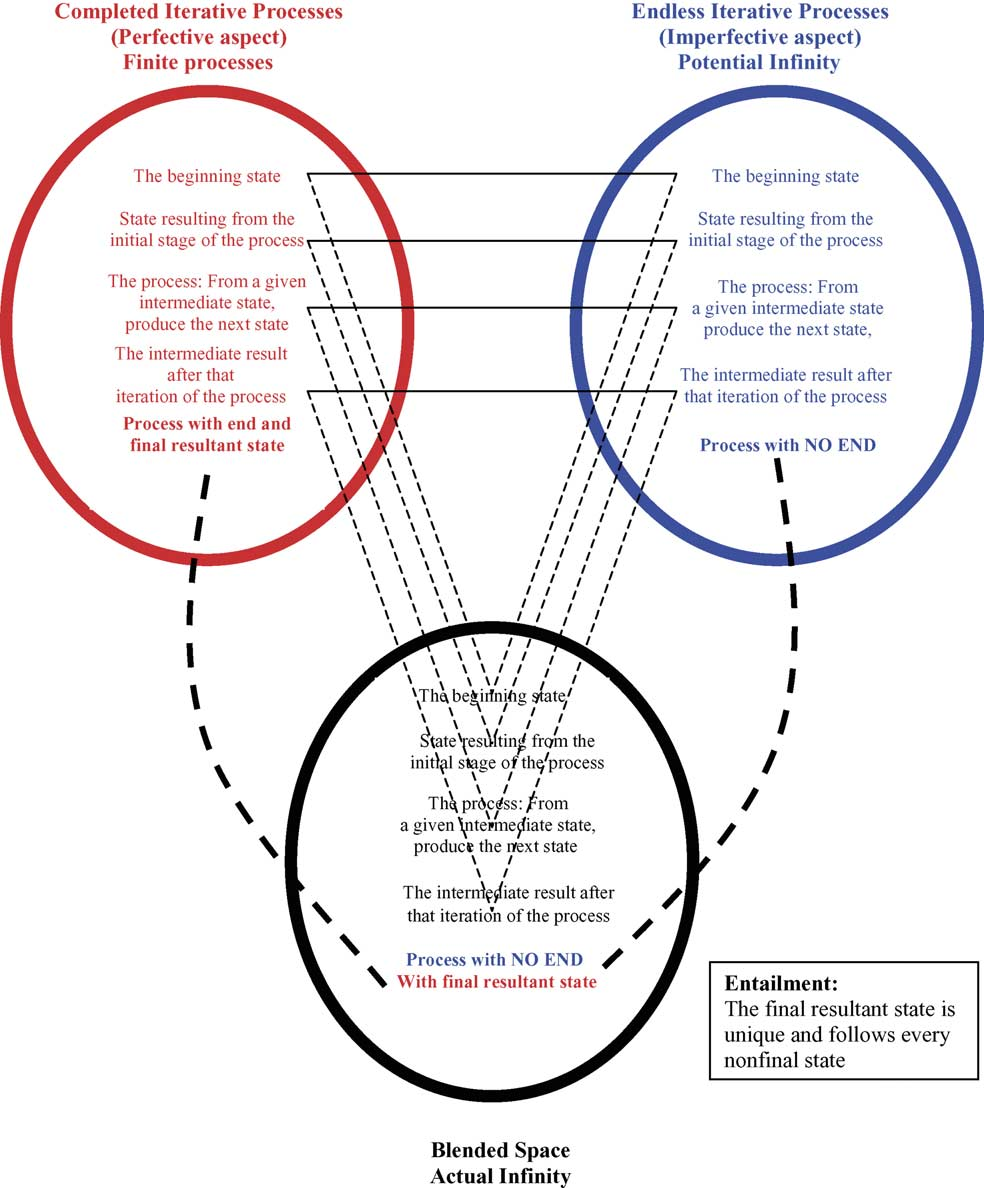
\includegraphics[width=0.4\textwidth]{transfin_nunez}  
  \caption{Blend from \textcite[p ??]{nunez05}}
  \label{fig:nunez_transfin}
\end{figure}

Figure~\ref{fig:nunez_transfin} gives an indication of the components
of the blend:
\begin{itemize}
\item The two input spaces at the top correspond to notions
of processes involving state change:
\begin{itemize}
\item  Completed Iterative Processes
are those that from some initial state, terminate in a final state
after a finite number of state transitions;
\item 
Endless Iterative Processes are those that continue indefinitely
to change state.
\end{itemize}
The marked correlations between features of the input spaces
indicate the common structure that is captured in our approach
by hte Generic Space, and as a result appear in the blend space.
\item 
Finally, the blend includes new features taken from both of the
input spaces, namely both ``process with no end'' and 
``final resultant state''.
\end{itemize}


%%% Local Variables: 
%%% mode: latex
%%% TeX-master: "mathsICCC"
%%% End: 
